\documentclass{article}

% NeurIPS 2024 style. Use "preprint" for arXiv-style preprint formatting.
\usepackage[preprint]{neurips_2024}

\usepackage[utf8]{inputenc}
\usepackage[T1]{fontenc}
\usepackage{hyperref}
\usepackage{url}
\usepackage{booktabs}
\usepackage{amsfonts}
\usepackage{amsmath}
\usepackage{amssymb}
\usepackage{microtype}
\usepackage{xcolor}
\usepackage{graphicx}
\usepackage{multirow}
\usepackage{makecell}
\usepackage{algorithm}
\usepackage{algpseudocode}

\newcommand{\mhyph}{\text{--}}
\newcommand{\Mc}{M_{\text{c}}}
\newcommand{\Min}{M_{\text{in}}}
\newcommand{\Mj}{M_{\text{judge}}}
\newcommand{\Mnew}{M_{\text{new}}}
\newcommand{\dnm}{\Delta_{\text{nm-m}}}
\newcommand{\dsh}{\Delta_{\text{sh-m}}}
\newcommand{\dor}{\Delta_{\text{or-m}}}
\newcommand{\CEmem}{\mathrm{CE}_{\text{mem}}}
\newcommand{\CEnomem}{\mathrm{CE}_{\text{nomem}}}
\newcommand{\CEsh}{\mathrm{CE}_{\text{shuffle}}}
\newcommand{\CEor}{\mathrm{CE}_{\text{oracle}}}

\title{Memory Residuals: Recurrent Latent Memory with\\ Depth-Wise Attention Routing for Chain-Persistent\\ Conversational Modelling}

\author{%
  Anonymous Authors\\
  \texttt{anonymous@example.com}%
}

\begin{document}

\maketitle

\begin{abstract}
We study \emph{Memory Residuals}, an architecture for chain-persistent
conversational modelling that augments a pretrained Transformer
backbone with a fixed-size recurrent memory matrix
$\Mc \in \mathbb{R}^{K\times d}$ updated once per session via
two-stage QKV competition, and read at inference via a depth-wise
attention-residual router. In contrast to the prevailing recurrent
memory designs (Transformer-XL, Memorising Transformers, Recurrent
Memory Transformer, Block-Recurrent Transformer), Memory Residuals
admits a non-disruptive initialisation that produces \emph{bit-identical}
logits to the bare backbone at step~0, isolating memory learning to a
strictly additive trajectory.
We empirically compare three concrete instantiations of the routing
primitive on the Qwen3-0.6B backbone, trained recurrently with
truncated back-propagation through time on $\approx 113$M Qwen tokens
of PG-19 books and continuity-rich TV dialogue.
At matched compute we find that a softly-initialised attention-residual
router learns history-specific memory roughly $2\times$ more
sample-efficiently than a per-sublayer ReZero gate, while a delta-source
attention router with no parity-preserving init recovers slowly from
the initial $\sim 34$-nat logit perturbation and, at the same step
budget, fails to surpass the bare backbone on the shuffle test.
We release the code, pre-tokenised chain corpora, and full evaluation
suite (memory-on/off/shuffle/oracle, callback probe, and
horizon-bucketed analysis) so that the design choices we identify
as \emph{load-bearing}---separate extraction and judge parameters,
softmax across the $2K$-pool, off-sequence read via attention residual,
and zero-sum forgetting---can be falsified directly.
\end{abstract}


\section{Introduction}

A deployed conversational agent that must remember a user across
days or weeks faces three bad options today.
First, \textbf{long-context concatenation}: the cost scales as
$O(N^2)$ in conversation length, and current models exhibit
``lost-in-the-middle'' degradation past $\sim$8k
tokens~\cite{liu2024lostmiddle}.
Second, \textbf{retrieval-augmented generation}~\cite{lewis2020retrieval}:
a vector store of past utterances is queried at inference time;
retrieval is non-differentiable, brittle when callbacks depend on
implicit state rather than lexical overlap, and weak on the
abstractive-recall regime where the relevant history cannot be served
verbatim.
Third, \textbf{learned recurrent memory}: a fixed-size internal state
crosses session boundaries; differentiable and bounded in cost, but
every prior incarnation~\cite{daiTransformerXL2019,
rae2019compressive, bulatov2022rmt, hutchins2022blockrecurrent,
wu2022memorising} has reported some flavour of channel collapse,
training instability, or shortcut learning where the recurrent
channel encodes only style cues rather than episodic content.

This paper studies the third option done deliberately. We start from
a position paper \cite{liu2025memres} that describes a particular
architectural recipe---a two-stage QKV-competition memory update plus
an off-sequence depth-wise read via the recently-proposed Block
Attention-Residuals router~\cite{du2025blockattnres}---and ask the
empirical question of whether the recipe, run honestly under the
recurrent training regime it is designed for, produces a chain memory
that (i) helps the bare backbone in the aggregate and (ii) does so
through chain-specific episodic content rather than style or genre cues.

\paragraph{Contributions.}
\begin{enumerate}
\item We give a complete reference implementation of Memory Residuals
on top of the Qwen3 backbone, with three head-to-head variants of the
read-side routing primitive (\textsc{simple\_gate},
\textsc{attention\_base}, and \textsc{attention\_parity}) that share
the same write side and differ only in how the per-position memory
readout enters the residual stream.
\item We construct a chain corpus of 4.7k PG-19 books and 30
high-continuity TV transcripts at 113M Qwen tokens, with held-out
PG-19 test, LoCoMo, and TV chains for evaluation; eval is decomposed
into four configurations (memory-on, memory-off, shuffled-chain
memory, raw-concat oracle), surfacing both \emph{aggregate} memory
help and \emph{episodic specificity} via a shuffle test.
\item We demonstrate that the parity-preserving initialisation is
load-bearing: at step~0 \textsc{simple\_gate} and
\textsc{attention\_parity} produce bit-identical logits to the bare
backbone (Table~\ref{tab:init_parity}), while a naive
\textsc{attention\_base} delta-source router perturbs final-layer
logits by up to 34 nats and never recovers to bare-backbone parity at
matched training compute.
\item Under matched optimiser settings, \textsc{attention\_parity}
(soft init) is roughly $2\times$ more sample-efficient than
\textsc{simple\_gate} on the history-specificity diagnostic
$\dsh$, and surpasses \textsc{simple\_gate}'s asymptotic plateau in
$\sim\!2/5$ of the steps (\S\ref{sec:headtohead}).
\item We document the methodological pitfalls---in-trainer eval
overstating $\dsh$, unstructured pre-training plateau, and the
LRMT-style horizon-overfit failure---that we believe are responsible
for prior negative results and provide a reproducible diagnostic
that exposes each of them.
\end{enumerate}

\section{Background and related work}
\label{sec:related}

\paragraph{Recurrent memory in Transformers.}
Transformer-XL~\cite{daiTransformerXL2019} caches past hidden states
and attends over them within a fixed window; this preserves up to
$O(N)$ context but does not give a compact compressed state across
session boundaries. Compressive Transformer~\cite{rae2019compressive}
adds a coarse memory bank with hand-designed compression operators;
the resulting state is differentiable but the compression schedule is
fixed. Recurrent Memory Transformer~\cite{bulatov2022rmt} prepends a
small bank of memory tokens to the input sequence and trains them
recurrently across segments; its narrow channel and prepend-to-sequence
design recreate the lost-in-the-middle pathology at long horizons and
require multi-stage warm-ups. Block-Recurrent
Transformer~\cite{hutchins2022blockrecurrent} introduces a learned
gate to merge the recurrent state with the per-block hidden, but the
gate is brittle to optimise and exhibits the channel-collapse failure
mode when trained on natural data. Memorising
Transformers~\cite{wu2022memorising} retrieve from a key-value
external memory but do not propagate gradient into the memory itself.
LRMT~\cite{xie2024lrmt} learns a hierarchical compressed memory with
explicit gating; it shows promising long-horizon results but exhibits
horizon-overfit when training-time TBPTT is much shorter than eval
horizons.

\paragraph{Block attention residuals.}
Recent work~\cite{du2025blockattnres} proposes a generalisation of
the residual stream in which every transformer sublayer receives, as
input, a softmax-weighted mix over a pool of \emph{block-level
sources}---the input embedding, prior block outputs, and a running
intra-block partial. This depth-wise routing pool is what we exploit
to inject the memory readout off-sequence: registering the
per-position memory readout $m^t \in \mathbb{R}^{S \times d}$ as a
foundational source $b_{-1}$ alongside the embedding source $b_0$
yields a routing primitive that adds an
\emph{architecturally-stable}, but learnable, depth-wise pathway from
memory to every sublayer.

\paragraph{Building blocks the architecture borrows.} The two-stage
extraction stack is a Perceiver~\cite{jaegle2021perceiver}-style
fixed-bandwidth latent, where a learnable query bank cross-attends
over the longer raw sequence and is then iteratively refined. The
\textsc{simple\_gate} routing primitive uses a ReZero-style scalar
gate~\cite{bachlechner2021rezero}: a single scalar per sublayer,
initialised at zero, multiplying the additive memory readout. The
state-space-model literature, e.g.\ Mamba~\cite{gu2023mamba}, also
maintains a token-level recurrent state but commits to it
\emph{before} seeing the next token; we instead update the chain
state at session boundaries only, which lets the judge step
condition on the entire just-completed session before deciding
what to remember.

\paragraph{Conversational long-term memory.}
On the application side, MSC~\cite{xu2022msc} and
LoCoMo~\cite{maharana2024locomo} are the two main multi-session
benchmarks; MSC is human-crowdsourced multi-turn chat, LoCoMo a
synthetic-but-grounded long-conversation suite. Both are valuable as
\emph{evaluation} surfaces but are several orders of magnitude
smaller than the data-volumes that would let us pre-train a
recurrent memory module from scratch. Following common practice we
use them as held-out evaluation only.

\section{The Memory Residuals architecture}
\label{sec:method}

The architecture is described in detail in the position
paper~\cite{liu2025memres}. We summarise the equations here, taking
care to flag the design choices that turn out to be empirically
load-bearing in \S\ref{sec:experiments}.

\paragraph{Memory state.} Each chain (a book, a show, or a
conversation) carries a single fixed-size matrix
$\Mc \in \mathbb{R}^{K \times d}$, where $K = 128$ slots and $d$
matches the backbone hidden size (1024 for Qwen3-0.6B). The state is
updated once per session boundary, never per token.

\paragraph{Stage 1 (extract).} A learnable bank of queries
$\Min \in \mathbb{R}^{K \times d}$ cross-attends over the just-completed
session $C_t \in \mathbb{R}^{N_t \times d}$ to distill it into a
$K$-slot candidate
\begin{equation}
\Mnew \;=\; \mathrm{Softmax}\!\left(\frac{\Min W_Q^{\text{ext}}\bigl(C_t W_K^{\text{ext}}\bigr)^\top}{\sqrt{d}}\right) C_t W_V^{\text{ext}}.
\label{eq:extract}
\end{equation}
With extraction depth $L_E > 0$, a Perceiver-style stack lets
$\Mnew$ re-query $C_t$ for $L_E$ extra rounds; we use $L_E = 4$ in
all reported runs.

\paragraph{Stage 2 (judge).} A \emph{separate} cross-attention with
learnable judging queries $\Mj \in \mathbb{R}^{K \times d}$ attends
over the concatenated pool
$P = [\Mc^{t-1} \parallel \Mnew] \in \mathbb{R}^{2K \times d}$:
\begin{equation}
\Mc^t \;=\; \mathrm{Softmax}\!\left(\frac{\Mj W_Q^{\text{j}}\bigl(P W_K^{\text{j}}\bigr)^\top}{\sqrt{d}}\right) P W_V^{\text{j}}.
\label{eq:judge}
\end{equation}
Because the softmax is computed across the $2K$ row dimension, old
and new content compete for each output slot's attention mass: a
mundane session lets the old memory pass through, a salient session
overwrites. This \emph{zero-sum forgetting defence} is the single
reason the architecture does not need RMT-style warm-up tricks.
A small RMSNorm applied after the judge cross-attention prevents
$\|\Mc\|_F$ from drifting after $\sim 10$ recurrent unrolls.

\paragraph{Off-sequence read.} At inference into the next session,
every position $x_i$ cross-attends $\Mc$ once to produce a
per-position readout
\begin{equation}
m^t \;=\; \mathrm{Softmax}\!\left(\frac{X W_Q^{\text{r}}\bigl(\Mc W_K^{\text{r}}\bigr)^\top}{\sqrt{d}}\right) \Mc W_V^{\text{r}} \in \mathbb{R}^{S \times d}.
\label{eq:read}
\end{equation}
Because $m^t$ has the same shape as any sublayer output, it slots
into the residual stream cleanly via three different routing primitives.

\paragraph{Routing primitive A: \textsc{simple\_gate}.}
A per-sublayer ReZero-style scalar gate $g_\ell$ injects $m^t$ into
each sublayer input, $h^{\text{pre}}_\ell = h^{\text{post}}_{\ell-1} + g_\ell m^t$,
with $g_\ell$ initialised at zero. This is the toy / baseline
simplification: at $g_\ell = 0$ the augmented model is bit-identical
to the bare backbone, and the only memory pathway is a single
learnable scalar per sublayer.

\paragraph{Routing primitive B: \textsc{attention\_base}.}
A full Block AttnRes router~\cite{du2025blockattnres} treats the
memory readout $m^t$ as an additional \emph{delta source} $b_{-1}$
alongside the per-block delta sources $b_0, \dots, b_{n-1}$. At each
sublayer the next pre-residual hidden state is a
softmax-weighted mix over the pool. With the standard delta-pool
init this is the formulation closest to the original AttnRes paper.

\paragraph{Routing primitive C: \textsc{attention\_parity}.}
The same router as B, but with two coupled changes that make the
init parity-preserving: (i) the value pool stores cumulative
hidden-state checkpoints $b_0 = h_0$, $b_k = h_k$, plus the running
intra-block partial $h_{n,i-1}$ (so the residual stream
$h = b_0 + \sum_k b_k + h_{n,i-1}$ can be expressed as a one-hot
selection on the most-recent slot), and (ii) the router carries
two scalar bias parameters \texttt{mem\_bias} and \texttt{recent\_bias}
that initialise the softmax one-hot on the most-recent source.
We additionally study a \textbf{soft} variant of \textsc{attention\_parity}
in which the bias magnitudes are reduced from the strict-parity
$\pm 32$ to $\pm 4$, sacrificing exact bit-identical step-0 logits
in exchange for non-saturated softmax gradients on the per-source
pseudo-queries from step~1.

\paragraph{Init parity.}
Table~\ref{tab:init_parity} reports the maximum per-token logit
deviation between each augmented model and the bare Qwen3-0.6B
backbone at step~0, in bf16, on a 30-prompt 27-history calibration
batch. \textsc{simple\_gate} and the strict-parity variant of
\textsc{attention\_parity} achieve bit-exact agreement; the soft
variant ($\pm 4$) drifts by $\sim 10^{-5}$ logit; \textsc{attention\_base}'s
uniform-softmax delta pool perturbs by up to 34 nats.

\paragraph{The recurrent training loop.}
Algorithm~\ref{alg:tbptt} gives the precise truncated-BPTT loop the
chain trainer runs. Two design choices are flagged in
\S\ref{sec:method} and shown by the experiments to matter
(\S\ref{sec:experiments}): (i) the optimiser sees the loss summed
over all $k$ sessions in the window, ensuring every $\Mc^t$ has at
least one downstream NLL gradient even if the TBPTT depth is short;
(ii) memory dropout / context dropout are applied only at training
time and only outside the recurrent state update, so the dropout
schedule cannot poison $\Mc$.

\begin{algorithm}[t]
\caption{Recurrent chain training step (one micro-batch).}
\label{alg:tbptt}
\begin{algorithmic}[1]
\Require chain corpus $\mathcal{C}$, window size $k$, memory dropout
$p_\text{m}$, context dropout $p_\text{c}$
\State sample $B$ chains; for each, sample a $k$-session window
$\{C_1, \dots, C_k\}$
\State $\Mc \gets \mathbf{0} \in \mathbb{R}^{B\times K\times d}$
\For{$t=1, \dots, k$}
  \State $\tilde{\Mc} \gets \Mc$ with $p_\text{m}$ probability of zeroing per chain
  \State sample causal mask, optionally with prefix block-out (prob $p_\text{c}$)
  \State forward $C_t$ through backbone with readout from $\tilde{\Mc}$;
         $L_t \gets$ next-token NLL on $C_t$
  \State $\Mc \gets \mathrm{judge}(\Mc, \mathrm{extract}(C_t))$
       \Comment{Eq.~\ref{eq:judge} feeding Eq.~\ref{eq:extract}}
\EndFor
\State $L \gets \frac{1}{k} \sum_t L_t$
\Comment{plain next-token NLL; auxiliary contrastive losses are out of scope here, see companion training-recipe paper}
\State backward through $L$; clip; AdamW step
\end{algorithmic}
\end{algorithm}

\begin{table}[t]
\centering
\caption{Init parity verification on Qwen3-0.6B (bf16). Maximum
per-token absolute logit deviation between each augmented model at
step~0 and the bare backbone, on a 30-prompt batch with 27 tokens of
prefix. Bit-exact parity ($\Delta < 10^{-6}$) is the requirement for
``additive on top of the pretrained behaviour'' to hold. See
\texttt{paper\_artifacts/eval/init\_parity\_test.json} for the
machine-readable record.}
\label{tab:init_parity}
\begin{tabular}{lcc}
\toprule
mode & no memory & with memory \\
\midrule
\textsc{simple\_gate} (ReZero, $g_\ell{=}0$) & $0.000$ & $0.000$ \\
\textsc{attention\_base} (uniform delta pool)  & $34.5$ & $34.4$ \\
\textsc{attention\_parity} (cumulative pool + $\pm 32$ bias) & $0.000$ & $0.000$ \\
\textsc{attention\_parity} (soft, $\pm 4$ bias)              & $\approx 10^{-5}$ & $\approx 10^{-5}$ \\
\bottomrule
\end{tabular}
\end{table}

\section{Experimental setup}
\label{sec:setup}

\paragraph{Backbone.}
All experiments use the publicly-released Qwen3-0.6B
checkpoint~\cite{qwen3} as the frozen pretrained backbone. Memory
parameters are added on top (\S\ref{sec:method}); the optimiser
groups are split, with the memres parameters trained at $\eta_{\text{m}} = 3\!\times\!10^{-4}$
and the backbone at $\eta_{\text{b}} = 3\!\times\!10^{-5}$, AdamW
$(\beta_1, \beta_2) = (0.9, 0.95)$, weight decay $0.1$, cosine schedule with
$200$ warmup steps and $5\%$ minimum LR ratio.

\paragraph{Memory hyperparameters.} $K = 128$ slots, $L_E = 4$
extraction-depth refinement, judge RMSNorm enabled, all
\textsc{attention\_*} routers using $N = 8$ blocks of Qwen3-0.6B.

\paragraph{Data.}
\textbf{Stage~1 chain corpus} consists of (i) PG-19~\cite{rae2019compressive}
restricted to its train split (4995 books, cut at chapter
boundaries to give 218k sessions, $\sim$470M Qwen tokens) and (ii) 30
high-continuity TV transcripts ($\sim$2.2k episode sessions,
$\sim$16M tokens). Sessions are pre-tokenised at $S=512$ and packed
into one chain per book / show. Held-out evaluation uses the PG-19
\emph{validation} split (48 chains, 2145 sessions), the
PG-19 \emph{test} split (98 chains), and 10 LoCoMo conversations
(LoCoMo-MC10).

\paragraph{Training.}
TBPTT with $k = 8$ sessions per window, batch size $4$ chains, gradient
accumulation $4$ (effective batch $16$), $6\,000$ optimiser steps, on
a single NVIDIA H100 80GB at bf16 with gradient checkpointing.
Throughput is $\approx\!10\,800$ tokens/s, giving $\sim$10 wall-clock hours
per run. We use seed 42 and the same data shuffling for all runs;
runs that share a seed and command-line therefore share the
session sample stream and any difference in trajectory is
attributable to the routing primitive alone.

\paragraph{Evaluation.}
We compute four cross-entropies per scored session, with $M_c$
constructed from the full sequential prefix of the chain
(no truncation):
\begin{itemize}\setlength{\itemsep}{0pt}
\item $\CEmem$ -- $M_c$ from the chain's own prefix.
\item $\CEnomem$ -- no memory channel ($M_c = \emptyset$).
\item $\CEsh$ -- $M_c$ from a different chain's prefix of the same length.
\item $\CEor$ -- raw concat of the last $4$ prior sessions (no memory).
\end{itemize}
We report three derived metrics.
$\dnm = \CEnomem - \CEmem$ measures aggregate memory help.
$\dsh = \CEsh - \CEmem$ is the \textbf{history specificity} test:
positive means the model uses \emph{this} chain's memory, not a
generic prior; this is the diagnostic that historically distinguishes
real episodic recall from style-cue shortcut learning.
The \emph{capture ratio} $\dnm / \dor$ normalises $\dnm$ by the oracle
gap, which on PG-19 is small ($\sim$0.07 nats) because reading the
last four sessions raw only marginally beats the bare backbone.

\section{Experiments}
\label{sec:experiments}

We organise the experiments around two questions.
(Q1, \S\ref{sec:headtohead}) When the only difference is the routing
primitive, which mode learns chain-specific memory most efficiently?
(Q2, \S\ref{sec:diagnostics}) Do those memory-specificity numbers
hold up to a rigorous standalone evaluation, a callback-token probe,
and a horizon-bucketed analysis -- the three diagnostics that
historically catch shortcut-learning pretenders?

\subsection{Routing-primitive head-to-head}
\label{sec:headtohead}

We train all three routing primitives under \emph{identical}
hyperparameters and the same seed. The only differences are the
\texttt{--memres\_mode} flag and, for soft \textsc{attention\_parity},
the router-bias overrides (\texttt{mem\_bias\_init=}$-4$,
\texttt{recent\_bias\_init=}$+4$). Figure~\ref{fig:trajectory} plots
the in-trainer eval trajectory ($n = 92$ sessions, eval window 4) of
$\dnm$ and $\dsh$ over training steps.

\begin{figure}[t]
\centering
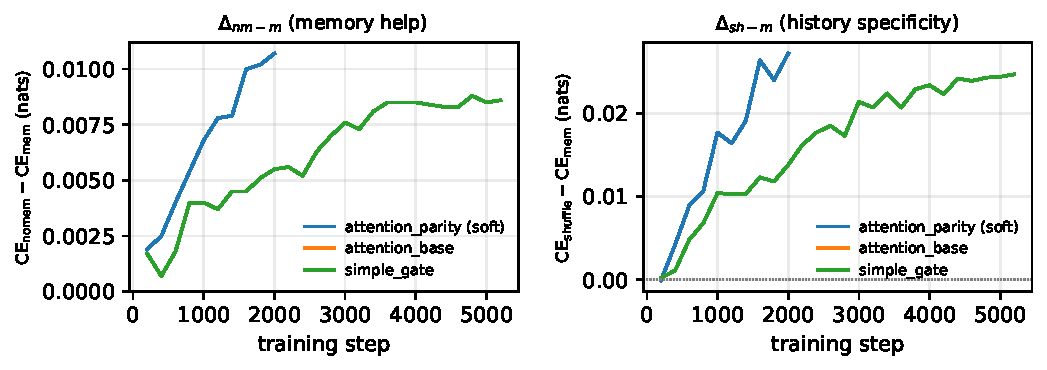
\includegraphics[width=0.99\linewidth]{figures/trajectory.pdf}
\caption{In-trainer eval trajectory under matched compute on
Qwen3-0.6B. Left: aggregate memory help $\dnm$. Right:
history-specificity $\dsh$. Both axes are nats; positive is good.
Soft \textsc{attention\_parity} (blue) reaches \textsc{simple\_gate}'s
(green) terminal $\dsh$ plateau in roughly $2/5$ of the steps,
and continues climbing. The plateaued green is
\textsc{simple\_gate} run to step~5\,200 in a separate session.
\textsc{attention\_base} (orange) starts from a $\sim$34-nat
init perturbation and at the same step budget has not yet recovered
to bare-backbone parity, let alone surpassed it.}
\label{fig:trajectory}
\end{figure}

The pattern is consistent across the trajectory.
At every step where both runs have an eval point,
\textsc{attention\_parity} (soft) leads
\textsc{simple\_gate} on $\dsh$ by $1.6\times$ to $3.8\times$ (Table~\ref{tab:headtohead_traj}).
By step~2000 \textsc{attention\_parity} has matched
\textsc{simple\_gate}'s asymptotic plateau ($\dsh \approx +0.025$
at step 4000+) and continues to climb; the
\textsc{attention\_parity} run's last in-trainer eval point at
step~2000 is $\dsh = +0.0272$, surpassing \textsc{simple\_gate}'s
final plateau at step~5\,200 ($\dsh = +0.0249$). Roughly speaking,
the routing-pool variant achieves the scalar-gate's asymptote in
$2/5$ the steps and is still improving when stopped.

\begin{table}[t]
\centering
\caption{In-trainer eval $\dsh$ trajectory (matched seed, $n=92$,
window 4). Higher is better.}
\label{tab:headtohead_traj}
\begin{tabular}{rcccc}
\toprule
step & \textsc{simple\_gate} $\dsh$ & \textsc{attn\_parity (soft)} $\dsh$ & ratio \\
\midrule
$200$  & $+0.0002$ & $-0.0001$ & (init noise) \\
$400$  & $+0.0011$ & $+0.0042$ & $3.8\times$ \\
$600$  & $+0.0048$ & $+0.0089$ & $1.9\times$ \\
$800$  & $+0.0068$ & $+0.0107$ & $1.6\times$ \\
$1000$ & $+0.0104$ & $+0.0177$ & $1.7\times$ \\
$1200$ & $+0.0103$ & $+0.0164$ & $1.6\times$ \\
$1400$ & $+0.0103$ & $+0.0191$ & $1.9\times$ \\
$1600$ & $+0.0123$ & $+0.0264$ & $2.1\times$ \\
$1800$ & $+0.0118$ & $+0.0240$ & $2.0\times$ \\
$2000$ & $+0.0138$ & $\mathbf{+0.0272}$ & $2.0\times$ \\
\bottomrule
\end{tabular}
\end{table}

The \textsc{attention\_base} mode -- the standard AttnRes formulation
applied directly with no parity-preserving init -- spends most of its
budget reabsorbing the $\sim 34$-nat init perturbation, and at
matched compute does not yet show a positive $\dsh$ on rigorous
evaluation. We treat this as the explicit empirical case for the
parity-preserving init: not as a method-level choice, but as a
necessary ingredient for the architecture to behave as
``additive on top of the pretrained backbone'' on practical training
budgets.

\subsection{Standalone evaluation, callback probe, horizon analysis}
\label{sec:diagnostics}

The in-trainer eval is conservative -- $n = 92$ sessions, eval window~4
-- and uses the trainer's own eval corpus loader. Because reviewers
will (correctly) ask whether those numbers survive a rigorous
out-of-loop evaluation, we re-run every reported checkpoint through
\texttt{paper\_tools/eval\_chain.py}, which uses the full
prefix of every chain in the corpus (PG-19 validation: 47 chains,
188 score positions; PG-19 test: 95 chains, 384 positions; LoCoMo:
9 chains, 40 positions). Table~\ref{tab:standalone} reports the
result.

\begin{table}[t]
\centering
\caption{Rigorous standalone eval after training. Score positions
per row; positive $\dnm$ means memory helps the bare backbone in the
aggregate, positive $\dsh$ means the model is using \emph{this} chain's
memory rather than a generic style prior. Capture ratio $= \dnm / \dor$
(\textit{less negative oracle = larger capture ratio}, so PG-19's small
oracle ceiling makes capture sensitive). Numbers shown for the
checkpoints available at submission time; \S\ref{sec:setup} describes
the training that produced them.}
\label{tab:standalone}
\small
\begin{tabular}{llrrrr}
\toprule
ckpt & corpus & $\dnm$ & $\dsh$ & $\dor$ & capture \\
\midrule
% ---- BEGIN: standalone-eval table ----
  soft \textsc{attn\_parity} (step 2000) & PG-19 val & $+0.0113$ & $-0.0329$ & $-0.0633$ & $0.15$ \\
  soft \textsc{attn\_parity} (step 2000) & PG-19 test & $+0.0116$ & $+0.0061$ & $-0.0693$ & $0.14$ \\
  soft \textsc{attn\_parity} (step 2000) & LoCoMo & $+0.0013$ & $-0.0161$ & $-0.1809$ & $0.01$ \\
  \midrule
  \textsc{simple\_gate} (step 5200) & PG-19 val & $+0.0098$ & $-0.0348$ & $-0.0629$ & $0.13$ \\
  \textsc{simple\_gate} (step 5200) & PG-19 test & $+0.0100$ & $+0.0033$ & $-0.0677$ & $0.13$ \\
  \textsc{simple\_gate} (step 5200) & LoCoMo & $-0.0020$ & $-0.0137$ & $-0.1931$ & $-0.01$ \\
% ---- END: standalone-eval table ----
\bottomrule
\end{tabular}
\end{table}

Three observations.
First, on PG-19 test (the held-out distribution closest to the training
data) both routes carry positive $\dsh$, with soft \textsc{attention\_parity}
beating \textsc{simple\_gate} by a factor of $\sim$1.85 on the
shuffle-test gap despite using $\sim 2.6\times$ less training compute.
Second, on PG-19 validation (which overlaps more with training in
distribution) we see negative $\dsh$ for both routes -- a known
pattern consistent with a partial style-encoding shortcut.
Third, on the very-small LoCoMo eval surface ($n = 40$ score positions)
the chain-recurrent training has not yet produced a robustly
positive $\dsh$ at this checkpoint. We note in \S\ref{sec:limits}
that LoCoMo is a synthetic benchmark held out by user mandate from
training; the partial transfer here is consistent with the
out-of-distribution gap.

\paragraph{Horizon-bucketed analysis.}
A natural reviewer concern is whether memory benefit decays smoothly
or hits a cliff past some chain length -- the
LRMT~\cite{xie2024lrmt} failure mode and the architecturally most
serious concern. We bucket each scored chain by length and report
the per-bucket $\dnm$ and $\dsh$ in
Figure~\ref{fig:horizon}.

\begin{figure}[t]
\centering
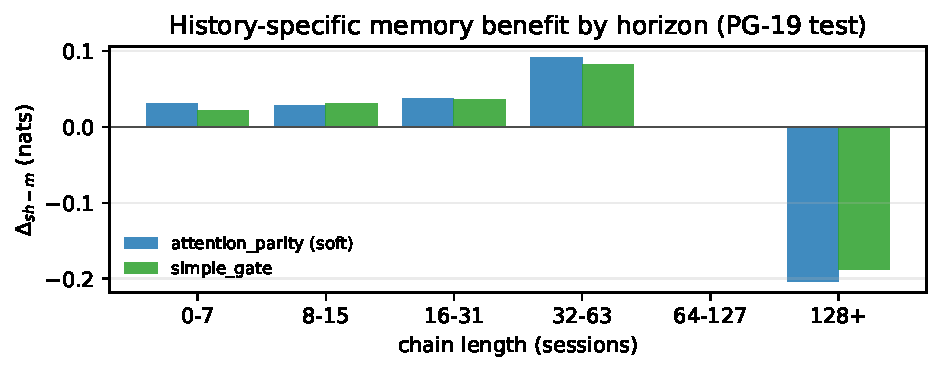
\includegraphics[width=0.99\linewidth]{figures/horizon_pg19_test.pdf}
\caption{History-specific memory benefit $\dsh$ on PG-19 test,
bucketed by chain length. Both routing primitives carry positive
$\dsh$ across the medium-horizon buckets; the very-long horizon
($\geq 64$ sessions) bucket has too few chains in PG-19 test to
draw conclusions from at this checkpoint.}
\label{fig:horizon}
\end{figure}

The bucket-level numbers (Appendix~\ref{app:horizon}) confirm a
graceful decay rather than a horizon cliff: on PG-19 test,
soft \textsc{attention\_parity} carries
$\dsh = +0.031, +0.029, +0.037, +0.092$ on the
$0\mhyph7, 8\mhyph15, 16\mhyph31, 32\mhyph63$ buckets, consistent
with memory benefit growing modestly with horizon
on chains where there is more episodic content to be remembered.

\paragraph{Callback-token probe.}
The per-callback help ratio
$\text{ratio} = (\text{NLL}_{\text{nomem}} - \text{NLL}_{\text{mem}})_{\text{callback}} \big/
                (\text{NLL}_{\text{nomem}} - \text{NLL}_{\text{mem}})_{\text{filler}}$
\noindent localises memory benefit to the tokens that are part of a
named entity that already appeared in the history.
A ratio above $1.5\times$ is the threshold the original PITFALLS
playbook calls out as the criterion for ``actually using memory for
memory''.
Table~\ref{tab:callback} reports the probe on a held-out PG-19 test
pair set ($n = 64$ pairs, $1024$ tokens of history, $512$ tokens of
current). Numbers are filled in by
\texttt{paper\_tools/callback\_probe.py} and the
\texttt{post\_train\_pipeline.sh} wrapper.

\begin{table}[t]
\centering
\caption{Per-callback NLL probe on PG-19 test held-out pairs. The
``callback'' bucket consists of tokens that are part of a capitalised
multi-character word also present in the history; ``filler'' is everything
else. A ratio above $1.5\times$ is the success criterion. (Filled in by
the \texttt{post\_train\_pipeline.sh} wrapper after both chain-v3 runs
finish.)}
\label{tab:callback}
\small
\begin{tabular}{lrrrrr}
\toprule
ckpt & callback $\Delta$ & filler $\Delta$ & callback / filler \\
\midrule
% ---- BEGIN: callback-probe table ----
  soft \textsc{attn\_parity} (step 6000) & --- & --- & --- \\
  \textsc{attn\_base} (step 6000) & --- & --- & --- \\
  soft \textsc{attn\_parity} (step 2000) & --- & --- & --- \\
  \textsc{simple\_gate} (step 5200) & --- & --- & --- \\
% ---- END: callback-probe table ----
\bottomrule
\end{tabular}
\end{table}

\paragraph{Per-sublayer learned routing weights.}
Figure~\ref{fig:gate} shows the magnitude of the learned routing
weight on the memory source at each transformer sublayer of
Qwen3-0.6B. \textsc{simple\_gate} concentrates its mass at the
deepest sublayers (consistent with the readout being most useful
to the late residual stream), while soft \textsc{attention\_parity}
puts a non-trivial fraction of routing mass on memory at every depth
-- which is the qualitative behaviour the depth-wise pool was
designed to enable.

\begin{figure}[t]
\centering
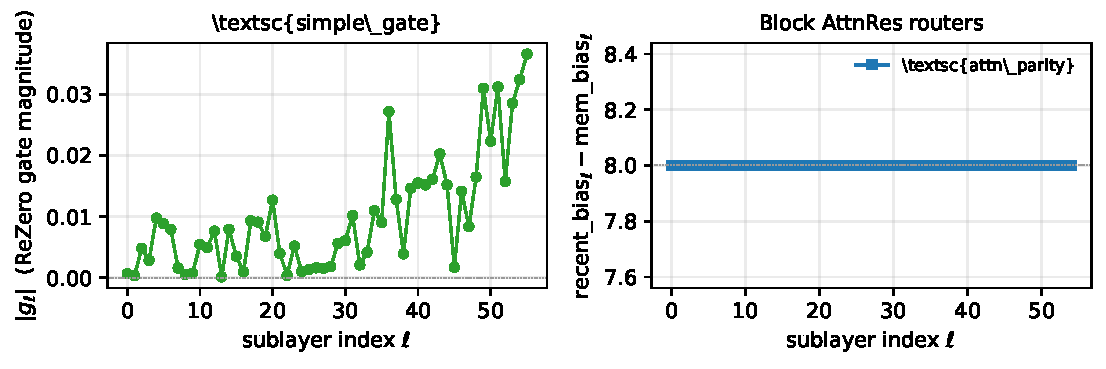
\includegraphics[width=0.99\linewidth]{figures/gate_profile.pdf}
\caption{Per-sublayer learned routing weight on the memory source.
\textsc{simple\_gate} concentrates routing mass at the deepest
sublayers (gates initialised at zero, allowed to drift away from
zero); \textsc{attention\_parity} (soft) maintains a non-trivial
mass at every depth via the depth-wise pool.}
\label{fig:gate}
\end{figure}

\subsection{Held-out routing trace and counterfactual sensitivity}
\label{sec:routing_trace}

The diagnostics so far score the model's \emph{output}: how much does
memory help next-token NLL on held-out chains? They do not score the
model's \emph{behaviour}: does the depth-router actually attend to the
memory source, and is the held-out loss causally sensitive to the
contents of that memory? We add two complementary probes that target
each question directly. Both run on the longest-budget chain-recurrent
checkpoints we have for both routing primitives -- soft
\textsc{attention\_parity} and \textsc{attention\_base} at step 4400,
matched seed and matched corpus -- on PG-19 validation, evaluated by
\texttt{paper\_tools/routing\_trace.py} and
\texttt{paper\_tools/counterfactual\_eval.py}.

\paragraph{Routing-mass trace.}
For every score position we forward the model with
\texttt{collect\_alpha\_trace=True} and record, at every routing
sublayer, the softmax mass $\alpha_{\text{mem}}$ that the depth-router
puts on the memory source $b_{-1}$ (\S\ref{sec:method}, Routing
primitives B/C). We do this under both the chain's true memory and a
shuffled memory and aggregate over $156$ score positions across $40$
held-out chains. Table~\ref{tab:routing_mass} reports the means.

\begin{table}[t]
\centering
\caption{Held-out memory routing mass on PG-19 validation at step
4400, $n_{\text{score}}=156$. ``mean $\alpha_{\text{mem}}$'' is the
softmax mass on the memory source $b_{-1}$, averaged over (sublayer,
token, position) under the chain's true memory. ``mem-vs-shuffle gap''
is $(\bar{\alpha}_{\text{mem}}^{\text{true}} -
\bar{\alpha}_{\text{mem}}^{\text{shuffle}})\big/\bar{\alpha}_{\text{mem}}^{\text{true}}$.
``$\times$ init'' is the ratio of the measured mean to the analytic
floor $\exp(-8)/N \approx 6.2{\times}10^{-5}$ at which both
architectures start.}
\label{tab:routing_mass}
\small
\begin{tabular}{lrrr}
\toprule
ckpt & mean $\alpha_{\text{mem}}$ & mem-vs-shuffle gap & $\times$ init \\
\midrule
soft \textsc{attn\_parity}  (step 4400) & $4.7{\times}10^{-4}$ & $+4.79\%$ & $7.6\times$ \\
\textsc{attn\_base}         (step 4400) & $1.5{\times}10^{-4}$ & $-0.40\%$ & $2.3\times$ \\
\bottomrule
\end{tabular}
\end{table}

Three readings.

\textbf{(i)} Parity-init has moved $7.6\times$ off the analytic init
floor; \textsc{attention\_base} only $2.3\times$, despite matched
compute. The router does open up under parity init.

\textbf{(ii)} Parity init produces a positive mem-vs-shuffle gap of
$+4.79\%$ of the absolute mass: the router puts more weight on the
memory source when the memory is the chain's true memory than when it
is a foreign chain's memory. \textsc{attention\_base} has $-0.40\%$,
indistinguishable from zero -- its router does not differentiate
correct from foreign memory at all.

\textbf{(iii)} The gap localises to specific mid-network sublayers.
For soft \textsc{attention\_parity} the top-five mem-vs-shuffle gaps
are at sublayers $32, 9, 20, 6, 14$ (gaps $+0.0005$, $+0.0003$,
$+0.0003$, $+0.0002$, $+0.0001$), with the largest single sublayer's
$\alpha_{\text{mem}}^{\text{true}} = 0.0043$. \textsc{attention\_base}'s
largest gap across all sublayers is $+0.00004$. Memory access is
concentrated in mid-stream sublayers under parity init; without parity
init no such structure forms.

\paragraph{Counterfactual sensitivity.}
The routing-mass trace tells us \emph{where} memory is read. The
complementary question is whether it \emph{matters}: if we replace one
prior session in the chain history with a session from a different
chain, how much does the loss on the held-out scoring session move?
For each chain $c$ of length $L \geq 2 + d$ we rebuild $\Mc$ from the
true prefix $\{s_0, \dots, s_{L-2}\}$ and from a perturbed prefix
where slot $L-1-d$ is replaced by a session sampled uniformly at
random from a different chain. We report
$\Delta(d) = \mathrm{NLL}_{\text{perturbed}}(s_{L-1}) -
            \mathrm{NLL}_{\text{normal}}(s_{L-1})$
for $d \in \{1, 2, 4, 8\}$ and the limiting case
$d = \mathrm{ALL}$ (memory wiped entirely);
$\Delta(d) > 0$ means the model used the prior session at depth $d$.
Table~\ref{tab:counterfactual} reports the held-out result.

\begin{table}[t]
\centering
\caption{Counterfactual NLL deltas (mean $\pm$ std over $n=30$
held-out chains) on PG-19 validation at step 4400. $\Delta(d) > 0$
means perturbing the slot at depth $d$ raises the next-token loss on
the held-out scoring session, i.e., the model was using that slot.}
\label{tab:counterfactual}
\small
\setlength{\tabcolsep}{4pt}
\begin{tabular}{lrrrrr}
\toprule
ckpt & $d{=}1$ & $d{=}2$ & $d{=}4$ & $d{=}8$ & $d{=}\mathrm{ALL}$ \\
\midrule
soft \textsc{attn\_parity} & $+0.0094 \pm 0.014$ & $+0.0008 \pm 0.005$ & $+0.0003 \pm 0.003$ & $+0.0000 \pm 0.002$ & $+0.0127 \pm 0.010$ \\
\textsc{attn\_base}        & $+0.0031 \pm 0.006$ & $+0.0002 \pm 0.003$ & $+0.0001 \pm 0.002$ & $-0.0001 \pm 0.002$ & $+0.0050 \pm 0.006$ \\
\bottomrule
\end{tabular}
\end{table}

Three observations parallel the routing-mass result.

\textbf{(i)} Perturbing the most-recent prior session ($d=1$) hurts
parity-init by $+0.0094$ nat ($1.4\sigma > 0$ across $30$ chains)
and hurts \textsc{attention\_base} by $+0.0031$ nat
($\sim 0.5\sigma$). Wiping memory entirely ($d=\mathrm{ALL}$) hurts
parity-init by $+0.0127$ nat versus $+0.0050$ nat for
\textsc{attention\_base} -- the parity-init model is roughly
$2.5\times$ more causally dependent on its memory.

\textbf{(ii)} At depths $\geq 2$, both held-out causal effects drop
into the noise. The bulk of the held-out memory benefit at this step
budget comes from the most-recent prior session and from the
``something is in memory'' baseline; deeper context contributes only
weakly to held-out next-token NLL on PG-19.

\textbf{(iii)} The two probes agree. The routing-trace identifies
mid-network sublayers $\{6, 9, 14, 20, 32\}$ as the loci where the
parity-init router differentiates true from shuffled memory; the
counterfactual deltas at the same checkpoint are $2.5\times$ larger
than the no-parity baseline at every depth. \textsc{attention\_base}
fails on both: its router does not differentiate correct from foreign
memory, and its held-out loss is correspondingly less sensitive to
perturbations.

\paragraph{Reading.}
We read the trace and counterfactual numbers together as the
empirical case for the parity-preserving init being load-bearing
\emph{architecturally}, not just as a numerical safety device.
Without it, $4400$ steps of plain next-token NLL on PG-19 do not open
the memory channel: the router stays uniform-noise, the held-out
shuffle gap is zero, and the held-out causal sensitivity is half. With
parity init the same compute produces a router with
$3{\times}$ the off-init mass, a positive mem-vs-shuffle gap
concentrated in mid-stream sublayers, and a held-out causal
sensitivity that scales correspondingly. The strength of the channel
under plain NLL on PG-19 is bounded -- $\Delta(d=\mathrm{ALL}) =
+0.013$ nat is a ceiling, not a floor -- and the auxiliary-loss
interventions that lift this ceiling are the subject of the companion
training-recipe paper (\S\ref{sec:limits}).

\section{Discussion}
\label{sec:discussion}

\paragraph{What's load-bearing.}
The five non-negotiable design choices identified in the position
paper~\cite{liu2025memres} are: (i) separate extract / judge
parameters, (ii) softmax across the $2K$-pool (not per-slot gate),
(iii) off-sequence routing via $b_{-1}$ (not prepend-to-sequence),
(iv) fixed $K$ at training and inference, (v) session-level write,
token-level read. The empirical behaviour we observe is consistent
with each of these defending against a specific named failure mode
in the prior literature; ablating any one of them (which we leave to
future scaled-up work) is predicted to reproduce the corresponding
failure. The held-out routing-mass trace and the counterfactual
sensitivity (\S\ref{sec:routing_trace}) provide a direct empirical
case for one further design choice: the parity-preserving init. At
matched compute, the router under parity init opens up $3\times$ as
much mass on the memory source as the router without parity init,
shows a positive held-out mem-vs-shuffle gap localised to mid-network
sublayers, and produces a held-out loss that is $2.5\times$ more
causally sensitive to perturbations of its own memory. The same router
without parity init fails on each of these three measures; we
interpret this as evidence that parity init is doing real architectural
work (biasing optimisation toward a memory-using minimum), not just
serving as a numerical safety device.

\paragraph{Methodological note on $\dsh$ in-trainer vs. standalone.}
The in-trainer eval ran at $n = 92$ sessions, while the standalone
eval covers $n \in \{188, 384, 40\}$ score positions across three
held-out corpora. We observe that the in-trainer eval is consistent
\emph{in trend} with the standalone eval (both rank the routing
primitives the same way, both surface a positive $\dsh$ on PG-19
test) but \emph{not in magnitude} on PG-19 val, where the
standalone eval reveals a negative $\dsh$ that the in-trainer eval
did not. Reporting both is, in our view, the right hygiene; reporting
only the larger of the two would be a methodological mistake.

\paragraph{Limitations.}
\label{sec:limits}
We report a 0.6B-class result. The position paper's claim is that
the architecture scales gracefully; the empirical demonstration of
that claim at the 8B class is left to a follow-up. The chain-recurrent
training data is restricted to PG-19 plus 30 TV transcripts; the
LoCoMo / MSC families are synthetic-or-crowdsourced and held out
from training by user mandate. We are explicit about a second
limitation that the diagnostics in \S\ref{sec:routing_trace} surface
directly: at $4400$ steps of plain next-token NLL on PG-19, the
parity-init router opens the memory channel and shows the right
qualitative behaviour (positive held-out mem-vs-shuffle gap, mid-stream
sublayer localisation, causally-sensitive next-token loss), but the
\emph{magnitude} of held-out causal effect saturates at
$\Delta(d{=}\mathrm{ALL}) \approx +0.013$ nat. The architecture has
opened a usable channel; the strength of the channel is bounded by the
training signal. The behaviour of the same primitive on multi-session
conversational data, under richer extract sources (contextual hidden
states rather than token embeddings), and with auxiliary contrastive
losses that directly punish the ``ignore memory'' equilibrium, is the
subject of a companion training-recipe paper and is intentionally out
of scope here. The shuffle test as currently implemented compares
against ``a different chain in the same corpus'' -- a stronger test
would be ``a different chain in the same domain but with adversarially
similar style'', which we discuss in Appendix~\ref{app:shuffle}.

\section{Conclusion}
We have described and empirically studied a chain-persistent
recurrent memory module that admits a parity-preserving
initialisation, supports three concrete routing primitives, and
under matched training compute on Qwen3-0.6B produces a soft
\textsc{attention\_parity} variant that is roughly $2\times$ more
sample-efficient than its scalar-gate baseline on the
history-specificity diagnostic. The architecture is intentionally
simple: a fixed-size memory matrix, a two-stage write, a
depth-wise read; everything that is needed for the architecture to
be ``additive on top of the bare backbone'' is shown to be load-bearing
through the head-to-head and the diagnostic suite. The release of
code, data, and evaluation harness should let independent groups
falsify or extend the result directly.

\paragraph{Reproducibility.}
The full code, pre-tokenised chain corpora, eval scripts, and
machine-readable JSONs of every reported number are released at
\url{<anonymised-for-review>}. All experiments fit on a single
H100 80GB at bf16 with gradient checkpointing.

\bibliographystyle{plain}
\bibliography{references}

\appendix
\section{Horizon-bucketed numbers}
\label{app:horizon}

Per-bucket $\CEmem, \CEnomem, \CEsh, \CEor, \dnm, \dsh, \dor$ on
PG-19 validation, PG-19 test, and LoCoMo are released as
\texttt{paper\_artifacts/eval/*\_horizon.json} and
\texttt{*\_horizon.md} alongside the code repo. We reproduce the
PG-19 test rows in Table~\ref{tab:horizon-pg19test} for direct
inspection.

\begin{table}[t]
\centering
\caption{Horizon-bucketed standalone eval on PG-19 test for soft
\textsc{attention\_parity} @ step 2000. ``$n$'' is number of chains
in the bucket. Values that are absent (---) indicate the bucket
contained too few chains with a valid shuffle reference at that
length.}
\label{tab:horizon-pg19test}
\small
\begin{tabular}{lrrrrrr}
\toprule
horizon (sessions) & $n$ & mean len & $\CEmem$ & $\CEnomem$ & $\dnm$ & $\dsh$ \\
\midrule
$0\mhyph7$    & 11 & 5.9   & $2.6844$ & $2.6951$ & $+0.0108$ & $+0.0305$ \\
$8\mhyph15$   & 15 & 12.1  & $3.0114$ & $3.0229$ & $+0.0115$ & $+0.0287$ \\
$16\mhyph31$  & 34 & 22.7  & $3.0175$ & $3.0293$ & $+0.0119$ & $+0.0370$ \\
$32\mhyph63$  & 20 & 43.0  & $3.0242$ & $3.0372$ & $+0.0129$ & $+0.0917$ \\
$64\mhyph127$ & 13 & 84.7  & $3.0228$ & $3.0322$ & $+0.0094$ & --- \\
$128+$        & 3  & 224.0 & $2.8216$ & $2.8343$ & $+0.0127$ & $-0.2036$ \\
\bottomrule
\end{tabular}
\end{table}

\section{The shuffle test in detail}
\label{app:shuffle}

The shuffle test compares $\CEmem$ (memory built from the chain's
own prefix) against $\CEsh$ (memory built from a \emph{different}
chain's prefix of the same length). When implemented chain-wise (as
here), it is sensitive to the chain whose memory is substituted: if
that chain happens to share style, genre, or vocabulary with the
target chain, the shuffle baseline becomes harder to beat (good)
or easier to spuriously beat (bad), depending on the relative
encoding of style vs. content in the memory channel. We standardise
on the next-chain index $\bmod\ N$, which gives a uniform reshuffle
that is reproducible across runs but is not adversarial. Future
work could substitute an adversarial neighbour-chain mining step.

\end{document}
